\section{Consultas compostas}

\begin{frame}[fragile]{Consultas compostas}

    \begin{itemize}
        \item Consultas simples podem ser combinadas em consultas compostas por meio do 
            operador '\code{prolog}{,}', que corresponde ao \textbf{e} lógico

        \item A sintaxe para consultas compostas é

            \inputsyntax{prolog}{codes/compound.pl}

        \item Se uma mesma variável aparece em mais de um predicado da consulta composta, ela 
            deve ter o mesmo valor em todos eles para que exista um casamento de padrão para a 
            consulta composta

        \item O escopo de uma variável lógica é uma consulta, seja simples ou composta

        \item Se a mesma variável é utilizada em consultas distintas, cada consulta tem sua 
            própria cópia da variável
    \end{itemize}
\end{frame}

\begin{frame}[fragile]{Consultas compostas}

    \begin{itemize}
        \item O processo de \textit{backtracking} é utilizado para tentar casar todos os 
            padrões, da esquerda para a direita

        \item Ele encerra (porta \code{prolog}{exit}) com sucesso apenas se ele sai do 
            predicado mais à direita com sucesso

        \item Neste caso, ele imprima o conjunto de variáveis cujas atribuições tornaram
            a consulta composta verdadeira

        \item Se uma consulta sai pela porta \code{prolog}{redo}, apenas as variáveis presentes 
            no predicado mais à direita são desatadas (as variáveis associadas aos predicados 
            anteriores permanecem atadas)

        \item Se a consulta falha para um dos predicados, ela falha como um todo

        \item O operador ponto-e-vírgula (`\code{prolog}{;}') força uma reentrada no
            último predicado pela porta \code{prolog}{redo}

    \end{itemize}

\end{frame}

\begin{frame}[fragile]{Visualização do fluxo para consultas compostas em Prolog}

    \begin{figure}[h]
        \centering
        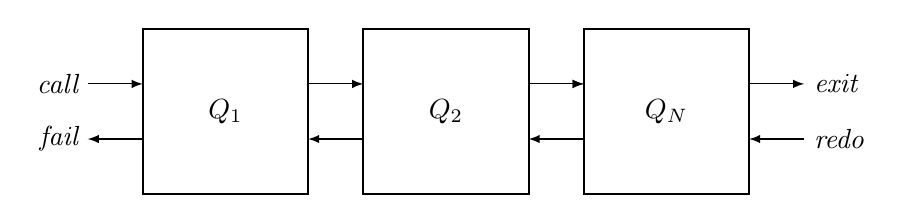
\begin{tikzpicture}[scale=0.7]
            \draw[thick] (0, 0) rectangle (3, 3);

            \draw[-latex] (-1, 2) node[anchor=east] {\it call} -- (0, 2);
            \draw[latex-] (-1, 1) node[anchor=east] {\it fail} -- (0, 1);
            \draw[-latex] (3, 2) -- (4, 2);
            \draw[latex-] (3, 1) -- (4, 1);
            \node at (1.5, 1.5) { $Q_1$ };

            \draw[thick] (4, 0) rectangle (7, 3);
            \draw[-latex] (7, 2) -- (8, 2);
            \draw[latex-] (7, 1) -- (8, 1);
            \node at (5.5, 1.5) { $Q_2$ };

            \draw[thick] (8, 0) rectangle (11, 3);
            \draw[-latex] (7, 2) -- (8, 2);
            \draw[latex-] (12, 2) node[anchor=west] {\it exit} -- (11, 2);
            \draw[-latex] (12, 1) node[anchor=west] {\it redo} -- (11, 1);
            \node at (9.5, 1.5) { $Q_N$ };


        \end{tikzpicture}
    \end{figure}

\end{frame}


\begin{frame}[fragile]{Exemplo de consultas compostas}

    \inputsnippet{prolog}{1}{21}{codes/capitais.pl}

\end{frame}

\begin{frame}[fragile]{Predicados pré-definidos}

    \begin{itemize}
        \item Prolog oferece uma série de predicados pré-definidos (\textit{built-in})

        \item Não há cláusulas para tais predicados

        \item Quando um objetivo casa com um predicado pré-definido, ele chama uma rotina 
            pré-definida

        \item Estas rotinas, em geral, são implementadas na mesma linguagem que implementou o 
            interpretador Prolog 

        \item Elas realizam tarefas que estão fora do contexto da prova de teoremas lógicos, 
            como escrever uma mensagem no console 

        \item Por esta razão, também são denominados predicados extra-lógicos 

        \item Ele respondem tanto na porta \code{prolog}{call} (\textit{left}) quando na 
            porta \code{prolog}{redo} (\textit{right})

        \item A resposta no caso \code{prolog}{redo} é denominada comportamento no 
            \textit{backtracking}

    \end{itemize}

\end{frame}

\begin{frame}[fragile]{Predicados extra-lógicos}

    \begin{itemize}
        \item Exemplos de predicados extra-lógicos de I/O:

        \begin{enumerate}
            \item \code{prolog}{write/1}: sempre casa com qualquer padrão, e tem como efeito 
                colateral escrever seu argumento no console. Sempre falha no
                \textit{backtracking}

            \item \code{prolog}{nl/0}: sempre é bem sucedido, e inicia uma nova linha. Também 
                falha no \textit{backtracking}

            \item \code{prolog}{tab/1}: avança $n$ espaços, onde $n$ é seu argumento. Mesmo 
                comportamento dos anteriores
        \end{enumerate}

            \item Estes predicados não afetam o fluxo de controle, transferindo-o controle 
                adiante (\textit{right}) ou para trás (\textit{backtracking})

            \item Eles também não alteram as variáveis

            \item O predicado \code{prolog}{fail/0} sempre falha

            \item Se ele recebe o controle vindo da esquerda, ele passa o controle 
                imediatamente para a porta \textit{redo} do objetivo à sua esquerda

            \item Ele nunca recebe o controle da direita, pois nunca deixa o fluxo avançar 
                para lá
    \end{itemize}

\end{frame}

\begin{frame}[fragile]{Exemplo de consultas que utilizam predicados extra-lógicos}

    \inputsnippet{prolog}{1}{21}{codes/quadrilaterals.pl}

\end{frame}
